%*******************************************************
% Capitulo cuatro
%*******************************************************

\chapter{Propuesta metodológica de producción}
\label{capitulometodologia}

El siguiente capítulo describe las dos categorías más fuertes en metodologías de desarrollo de software y realiza un análisis de las caracteristicas que afectan la decisión de escoger una u otra. Al final se plantean alternativas de selección a la metodología y se discute su escenario de aplicación.

\section{Metodologías de construcción de software}

Se realiza la construcción de una pieza software para el caso de estudio descrito en el capítulo \ref{Caso_de_estudio}. Este caso de estudio tiene las siguientes restricciones identificadas en su proceso de producción:

\begin{itemize}

    \item La metodología de trabajo empleada por el grupo fue creación coletiva. El proceso ocurre a lo largo de diferentes talleres en los que se hacen actividades de lectura, conversatorios y lluvias de ideas acerca de la muestra. En cada taller se hacen propuestas de trabajo y modificaciones que son valoradas por el grupo. Los requerimientos cambian ante cualquier idea rápidamente aceptada por el grupo.

    \item El proceso debe involucrar una sensibilización acerca de la presencia de la tecnología en el resultado final. El conocimiento de los usuarios de la tecnología se resume en lo tradicional: pantallas, televisores, proyectores y teclados. Todos deben volverse partícipes del proceso de innovación a persar que no tengan conocimientos en tecnología.

    \item Se deben hacer iteraciones frecuentemente. La construcción debe permitir entregas rápidas que le permitan a los miembros del grupo tomar decisiones frente a los construido para evitar reprocesos o que se acepten ideas distantes de lo diseñado previamente.

    \item El fin de los talleres de construcción puede ser otro al de diseñar la obra, por ejemplo describir memorias del pasado o crear piezas físicas para la obra final, por lo que se presenta confusión entre los participantes cuando se les habla de tecnología. Se debe analizar como establecer de forma clara reuniones que funcionen en el marco de alguna metodología que no sea exclusivamente para proyectos de desarrollo de software.

    \item El proceso debe incluir una documentación de contexto para crear un vocabulario común entre los participantes.

\end{itemize}

La construcción de las piezas software y de la infraestructura de tecnología estará a cargo del autor de éste trabajo. Se proponen durante los talleres las piezas de infraestructura para que todos los participantes tengan claro qué deben incluir en los procesos de creación.

Durante el proceso, debe haber reuniones de aprobación de los avances para tomar decisiones de construcción o corrección, en éstas se debe tener en cuenta la opinión de todo el grupo.

Se determina entonces que el alcance es variable para este proyecto. En el proceso creativo se realizan cambios constantes al producto final y la cantidad de mano de obra requerida puede cambiar drásticamente. El costo y el tiempo son limitados porque los recursos utilizados tienen un tope finito; se establece que hay una restricción de tiempo fijo, costo fijo y alcance variable.

\section{Selección de la metodología}

Se propone el uso de la metodología SCRUM como base para realizar un propuesta metodológica de construcción de software.

\subsection{Puntos en común}

Entre las razones para escoger como punto de partida SCRUM está:

\begin{itemize}
  \item La tripe restricción: alcance, tiempo y costo; en este proyecto el alcance es variable mientras el tiempo y el costo son fijos. SCRUM es una metodología de alcance variable.
  \item Scrum tiene reuniones especilizadas que podrían servir de base para este proyecto.
  \item Scrum tiene consideraciones especiales acerca de las entregas de valor que permiten tener una evolución visible del proyecto desde el principio.
\end{itemize}

\subsection{Diferencias}

Se deben tener en cuenta las siguientes consideraciones:

\begin{itemize}

  \item La construcción colectiva comienza al mismo tiempo que el proyecto de software, durante el inicio se deben construir piezas que alimenten el imaginario colectivo del resultado final, pero desde el principio no se conoce casí ningún detalle del resultado. No existe una versión inicial del \textit{product backlog}.

  \item Las reuniones de Scrum no están diseñadas para discutir temas que no sean software. La definición de los requisitos se convierte en un trabajo del día a día del \textit{product owner}.

  \item Raramente las entregas de valor tienen que ver con temas diferentes a software. En éste proyecto la usabilidad, las pruebas y el comportamiento de todo el sistema va más allá de las entregas de valor: los factores humanos son más exigentes.

  \item El equipo no es maduro. Hay muchas disciplinas diferentes involucradas durante el proceso de construcción de software.

\end{itemize}

\subsection{Propuesta de modificación}

Se establecen las siguientes propuestas de trabajo que modifican la estructura original de Scrum. Algunos autores como \cite{peixoto2009human, moreno2012agile, nielsen2008agile} han discutido acerca de las vntajas y desventajas del uso de metodologias ágiles en el desarrollo de historias de usuario. Una lista de los problemas sobre la construcción de las historias de usuario es explicada por \cite{peixoto2009human} y describe como la separación entre el lenguaje escrito y los elementos visuales o táctiles de la usabilidad pueden causar problemas durante el proceso de desarrollo. Se proponen entonces cambios metodológicos a la versión oficial de la metodología ágil intentando mitigar algunos de los problemas descritos por el estado de arte.

\subsubsection{Roles de Scrum}

Tradicionalmente se tienen tres roles: \textit{Scrum Master}, \textit{Product owner} y \textit{Developer}; se propone la siguiente estructura modificada:

\begin{itemize}

  \item Se mantiene el \textit{scrum master} para realizar la guía fundamental y resolución de inconvenientes que plantea la metodología. El Scrum master tendrá una función adicional: Deberá construir el vocabulario común de comunicación con el resto del equipo de no desarrolladores.

  \item El \textit{product owner} tiene mayores responsabilidades en la definición y defensa del producto backlog. Para garantizar que los esfuerzos en construcción nunca se pierdan se debe  hacer una revisión permanente de que el product backlog siempre esté actualizado con los conceptos comúnmente aceptados. El product owner responde por la búsqueda del acuerdo global y resuelve las diferencias entre los miembros del equipo en cuanto a la definición del producto software.

  \item El rol de \textit{developer} se mantiene con un elemento adicional, debe participar de la creación colectiva aportando ideas que permitan que los artistas construyan desde el conocimiento real de la tecnología. El desarrollador de software no puede ser nada más un espectador del proceso creativo, debe ser protagonista y debe crear a la par de los miembros del colectivo de arte.

\end{itemize}

\subsubsection{Actividades de Scrum}

Las reuniones de Scrum son importantes en su estructura y deben mantenerse. Se proponen los siguientes cambios a algunas de las reuniones:

\begin{itemize}

  \item \textit{Sprint planning meeting}. Las reuniones de planeación del inicio de la iteración se mantienen en su forma fundamental. Se deben realizar dos cambios importantes: 1) La reunión debe ser antecedida por los talleres de trabajo regulares. En estas se establece el product backlog de la ciclo y se necesitan un insumo adicional para interpretar la información entregada por el artista. 2)  Es fundamental la presencia en la reunión de personas que no sean desarrolladores.

  \item \textit{Daily Scrum}. La reunión diaria se mantiene y es un eje importante del proceso para poder resolver las dudas del contexto. La producción diara debe ser verificada casí de forma inmediata. Se podrían repetir varias veces al día las reuniones para garantizar que no haya desviación de los planes que tienen alta volatilidad.

  \item \textit{Sprint Retrospective}. La reunión de revisión permite resolver diferentes conflictos de infraestructura o talento humano diferentes al desarrollo del product backlog. Hay que resolver todos los inconvenientes relativos al desarrollo de interfaces de usuario.

  \item \textit{Sprint}. La iteración para este tipo de proyectos se propone sea de una semana únicamente debido a la alta variabilidad del \textit{product backlog}.

\end{itemize}

\subsubsection{Elementos de Scrum}

El elemento más complicado de gestionar desde la metodología ágil son las historias de usuario. La gestión de historias se realiza usualmente describiento elementos de entrada salida que representan flujos de información y acciones del usuario frente a un sistema, siendo los más típicos aquellos en donde se debe interactuar con formularios. Sistemas diferentes a los formularios con componentes interactivos más complicados suelen complicar también la forma y la precisión con la que la historia de usuario queda descrita, haciendo más dificil su seguimiento. La incertidumbre acerca de su entendimiento y la separación entre lo escrito y su realidad son un grave problema que no solo se presenta a ete nivel de construcción sino también el el desarrollo de cualquier sistema de HCI. Autores como \cite{moreno2012agile}, describen las características que debería tener un \textit{product backlog} al momento de incluir detalles de usabilidad.

Sin embargo, muchos de sus conceptos no pueden ser traídos a este contexto porque no existen los mismos componentes gráficos como botones, menús o cajas de selección. Existe la misma situación en el diseño de video juegos en los que diferentes autores también han desarrollado metodologías propias para diseñar y desarrollar sus productos. A pesar de todas las anteriores recomendaciones se propone seguir la estructura tradicional, extendiendo e implementando las sugerencias de \cite{moreno2012agile} y descartando las consideraciones relativas a componentes de interfaz gráfica no usados.

\begin{figure}[h]
\label{togafarchimate}
\centering
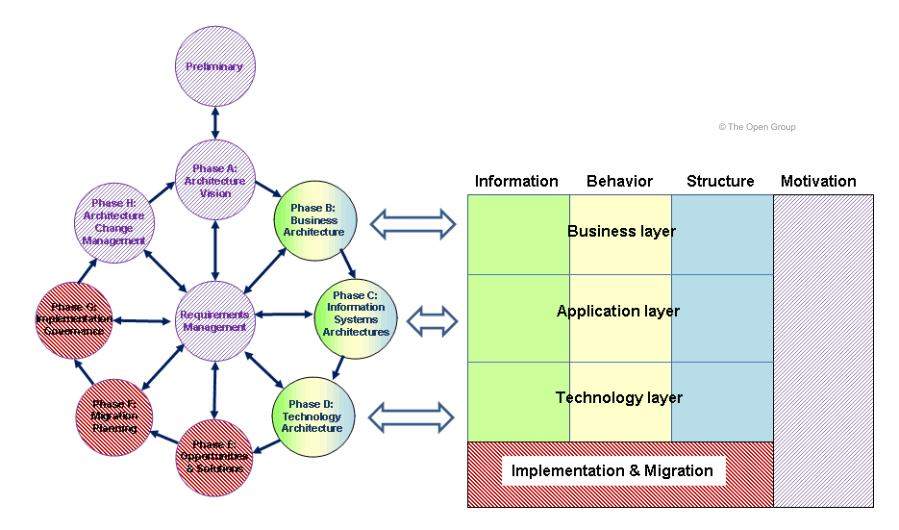
\includegraphics[scale=0.8]{togafarchimate}
\caption{Correspondencia entre Archimate y TOGAF.}
\end{figure}

Las entregas de valor al final de cada ciclo se mantienen como prototipos alterables en el futuro. Tradicionalmente, las entregas de valor son inalterables luego de revisadas y aprobadas, siendo cambiadas en las correcciones de bugs y en su integración con otras historias de usuario. En este caso se propone que cada incremento potencial tenga el alcance necesario, incluso con la modificación total o parcial de historias previamente entregadas y validadas.

El refinamiento de las historias de usuario debería tener dos etapas: 1) la documentación de nuevas ideas en el proceso regular de descubrimiento de nuevas ideas durante el proceso y, 2)la transformación de las historias de usuario recolectadas en nuevas historias con revisión y aprobación grupal.
